\section{Environment}
\label{mls:environment}

A multi-level secure database is much like any traditional database system. The major difference is the presence of resources, users, and transactions with differing security levels. This can be resources within the system that contain a certain a security level. This can also be true for users who maintain a certain security level and therefore the transactions generated by the user contains a certain security level. Current architecture solutions leverage the Bell-LaPadula model (\cite{bell_secure_1973}) to ensure that current security levels are maintained and data is not accessed inappropriately. The Bell LaPadula Model abides by two main rules to ensure secure data access. The two rules are:

\begin{enumerate}
  \item A subject at a given security level may not read an object at a higher security level. This is known as the Simple Security Property
  \item A subject at a given security level many not write to any object a lower security level. This is known as the * (star) Property
\end{enumerate}

\begin{figure}
\centering
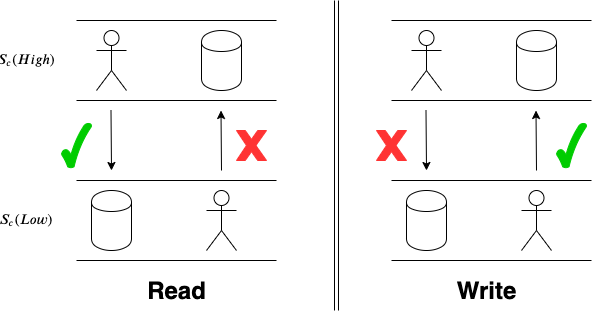
\includegraphics[scale=0.45]{images/BellLapadulaModel.png}
\caption{Bell-LaPadula Model}
\label{fig:bell_lapadula_model}
\end{figure}

Both of these properties are shown in Figure \ref{fig:bell_lapadula_model}. While this ensures proper data access control for security levels, the Bell-LaPadula Model doesn't protect against covert channels that occur due to concurrent transactions. Concurrent transactions cause issues when there are conflicting operations. When there is a conflict, one of the transactions must wait for the other transactions to finish processing before execution can continue processing. The presence (or even absence) of a time delay for the transaction to execute introduces a covert channel. 

A covert channel is a security flaw where a means of communication to transmit unauthorized information is available via the normal means of communication. Timing channels are a form of covert channel where the presence of absence of a execution delay conveys unauthorized information about the underlying system. This work is documented by Girling in \cite{girling_covert_1987}. Timing channels are difficult to prevent and many times requires review of the application source code directly to ensure all operations execute with the same timing delay. Common solutions to prevent covert timing channels in multi-level secure databases when there are conflicting operations is to abort the transaction with a higher security classification. This prevents the transaction with a lower security transaction from detecting a timing delay. The timing delay would communicate to the lower security transaction that resources of a higher security classification were present and therefore leaking unauthorized information. Figure \ref{fig:env_covert_channel_exposure} (referenced from Figure \ref{fig:ws_trans_starvation} in Section \ref{mls:problem_definition}) shows the exposure of a timing covert channel.

\begin{figure}
\centering
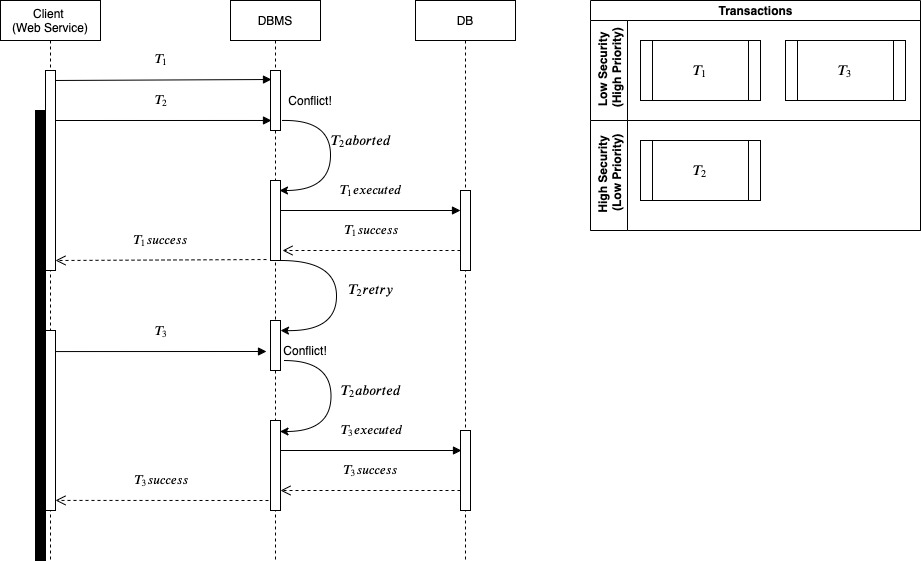
\includegraphics[scale=0.45]{images/TransactionStarvation.jpg}
\caption{Transaction Starvation Exposes Timing Covert Channel}
\label{fig:env_covert_channel_exposure}
\end{figure}